We begin by examining the case of a fixed model size with increasing input name counts, shown in \strongfigref{result:1} below. 

Our PC method outperforms all other baselines across every input size benchmarked. For both SC and UT, this result is unsurprising, as PC is more heavily optimized for this specific workload. More notably, PC also outperforms BT, which is a highly optimized and widely used ML framework. This advantage can largely be attributed to Python overhead in BT, including costs associated with object management and data movement between Python and underlying implementations.

However, a closer examination of the results shows that, while PC currently outperforms BT, its runtime increases more rapidly with input size, whereas BT exhibits near-ideal scaling behavior. It is therefore reasonable to expect that as input sizes continue to grow, particularly to those typical of modern ML workloads, PC will eventually lose its performance advantage.

\begin{figure}[h]
    \centering
    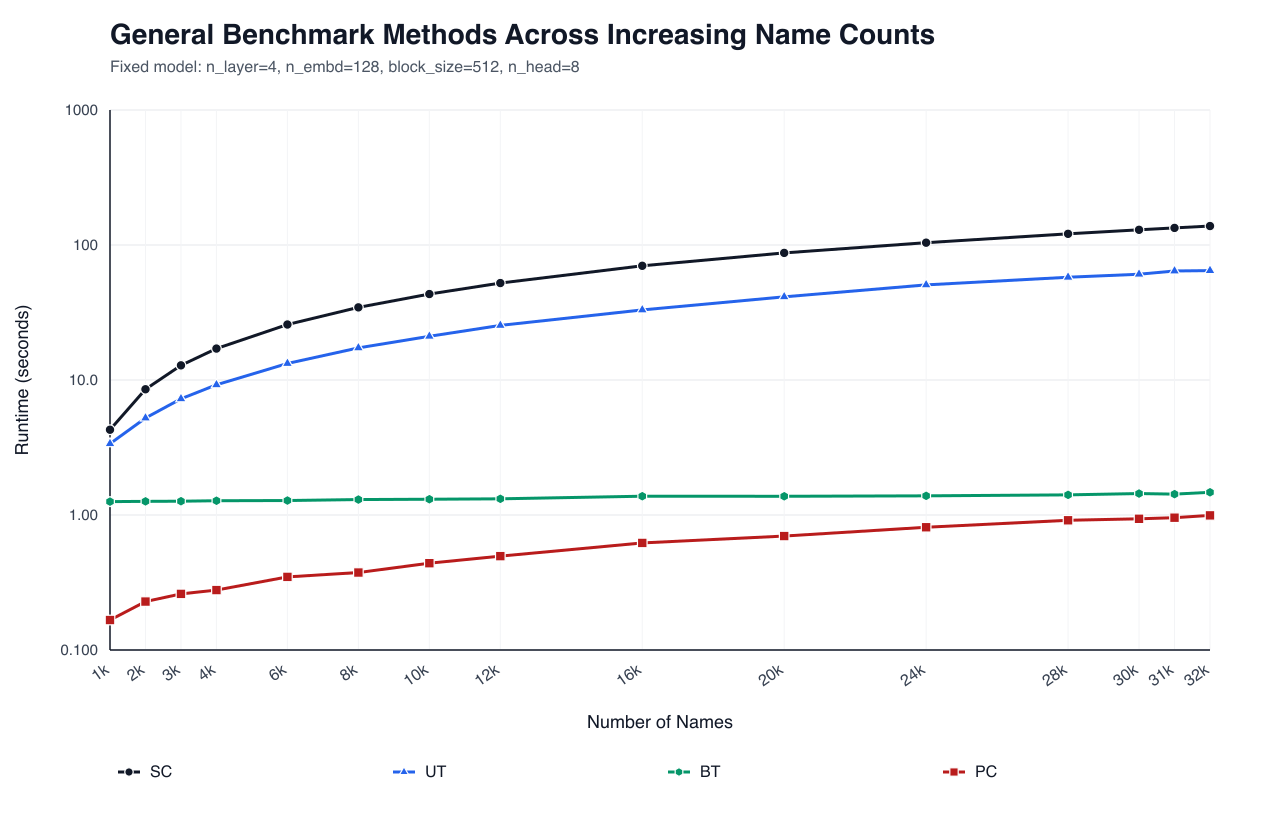
\includegraphics[width=\linewidth]{figures/general_benchmark_names.png}
    \caption{Results from Input Scaling}
    \label{result:1}
\end{figure}


Next we will look at the results from the other two scaling regimes: holding input size constant while increasing model size (ii), and increasing both input size and model size together (iii). The preset definitions for these experiments cam be found in \strongappref{appendix:presets} and the results are shown in \strongtabref{tab:model_configs}.




\begin{table*}[t]
\centering
\small
\begin{minipage}{0.49\textwidth}
\centering
\begin{tabular}{l c c c c}
\toprule
\textbf{Preset} & \textbf{UT} & \textbf{BT} & \textbf{SC} & \textbf{PC} \\
\midrule

MS5 & \makecell{4.33 \\ $0.28\times$}
    & \makecell{0.92 \\ $1.34\times$}
    & \makecell{1.23 \\ $1.00\times$}
    & \makecell{0.20 \\ $6.22\times$} \\

MM5 & \makecell{6.81 \\ $1.58\times$}
    & \makecell{1.10 \\ $9.80\times$}
    & \makecell{10.76 \\ $1.00\times$}
    & \makecell{0.26 \\ $41.38\times$} \\

ML5 & \makecell{12.45 \\ $7.51\times$}
    & \makecell{2.37 \\ $39.45\times$}
    & \makecell{93.53 \\ $1.00\times$}
    & \makecell{0.50 \\ $185.50\times$} \\

MVL5 & \makecell{20.20 \\ $16.21\times$}
     & \makecell{5.79 \\ $56.50\times$}
     & \makecell{327.28 \\ $1.00\times$}
     & \makecell{1.07 \\ $307.03\times$} \\

MXL5 & \makecell{32.29 \\ $24.30\times$}
     & \makecell{12.34 \\ $63.59\times$}
     & \makecell{784.64 \\ $1.00\times$}
     & \makecell{2.10 \\ $373.60\times$} \\


\bottomrule
\end{tabular}
\end{minipage}
\hspace{0.001\textwidth}  % adjust this
\begin{minipage}{0.48\textwidth}
\centering
\begin{tabular}{l c c c c}
\toprule
\textbf{Preset} & \textbf{UT} & \textbf{BT} & \textbf{SC} & \textbf{PC} \\
\midrule


S  & \makecell{2.30 \\ $0.22\times$}
   & \makecell{0.93 \\ $0.54\times$}
   & \makecell{0.50 \\ $1.00\times$}
   & \makecell{0.14 \\ $3.50\times$} \\

M  & \makecell{6.66 \\ $1.62\times$}
   & \makecell{1.07 \\ $10.04\times$}
   & \makecell{10.76 \\ $1.00\times$}
   & \makecell{0.25 \\ $42.40\times$} \\

L  & \makecell{23.32 \\ $8.14\times$}
   & \makecell{2.41 \\ $78.82\times$}
   & \makecell{189.75 \\ $1.00\times$}
   & \makecell{0.76 \\ $250.21\times$} \\

VL & \makecell{64.90 \\ $20.68\times$}
   & \makecell{6.14 \\ $218.60\times$}
   & \makecell{1342.22 \\ $1.00\times$}
   & \makecell{3.06 \\ $438.44\times$} \\

XL & \makecell{127.71 \\ $37.37\times$}
   & \makecell{13.46 \\ $354.55\times$}
   & \makecell{4771.83 \\ $1.00\times$}
   & \makecell{9.18 \\ $519.91\times$} \\

\bottomrule
\end{tabular}
\end{minipage}

\caption{Runtime (top)/speedup (bottom) per method. \textbf{Runtime is in seconds; Speedup is relative to SC}}
\label{tab:model_configs}
\end{table*}

Across both regimes, PC consistently outperforms all baselines, maintaining the largest speedup across almost every preset. This trend holds even as model size increases, demonstrating that the implementation effectively exploits parallelism in the dominant compute paths.

To better interpret these results, we define the forward-pass complexity as $O\bigl(N \cdot L \cdot (C_{\text{attn}} + C_{\text{mlp}})\bigr)$, where $C_{\text{attn}} = T^{2} \cdot d$ and $C_{\text{mlp}} = T \cdot E^{2}$. 
Under the assumption that $T$ remains approximately constant, this simplifies to $\approx O(N \cdot L \cdot d^{2})$.

The empirical trends in \strongtabref{tab:model_configs} align with this analysis. In regime (ii), where $N$ is fixed and model size increases, runtime grows rapidly with $d$ and $L$, consistent with the $d^{2}$ dependence. In regime (iii), where $N$, $L$, and $d$ all increase, the combined effect leads to the largest runtimes, reflecting the multiplicative $O(N \cdot L \cdot d^{2})$ scaling. Despite this growth, PC maintains a consistent advantage.

Overall, PC consistently outperforms all baselines while exhibiting scaling behavior that aligns with the theoretical $O(N \cdot L \cdot E^{2})$ complexity. However, BT demonstrates more favorable scaling at larger sizes, suggesting that PC's performance advantage may diminish for sufficiently large workloads.
